\subsection{The Billiard Lays a Golden Egg}
\label{sec:x40}

The {\em Bevan Point} $X_{40}$ is known as the Circumcenter of the Excentral Triangle \cite{etc}. It is the tangential polygon to the 3-periodic, and can be thought of as its projective dual \cite{levi2007-poncelet-grid}.

We have shown elsewhere the locus of $X_{40}$ is an ellipse similar to a rotated copy of the Billiard. Its semi-axes are given by \cite{garcia2020-ellipses}:
%
\begin{equation*}
    a_{40}=c^2/a,\;\;\; b_{40}=c^2/b.
\end{equation*}
%
\begin{proposition}
At $a/b=\sqrt{2}$ i.e., the top and bottom vertices of the $X_{40}$ touch the Billiard's top and bottom vertices.
\end{proposition}

\begin{proof}
This follows from imposing $b_{40}=b$.
\end{proof}

\noindent What we got next was unexpected, see Figure~\ref{fig:x40-golden}:

\begin{proposition}
At $a/b = (1+\sqrt{5})/2=\varphi$, the Golden Ratio, the locus of $X_{40}$ is identical to a $90^\circ$-rotated copy of the EB
\end{proposition}

\begin{proof}
This follows from imposing $b_{40} = a$.
\end{proof}

\begin{remark}
Let $A$ be area of the four-corner region common to an ellipse and its $90^\circ$-rotated copy. It can be shown $A/A_{ell}=4 \csc^{-1}\left[{\sqrt{1 + (a/b)^2}}\right]/\pi$, where $A_{ell}=\pi{a}{b}$, is the area of the ellipse. For $a/b=\varphi$, $A/A_{ell}{\simeq}0.704833$.
\end{remark}

\begin{figure}
    \centering
    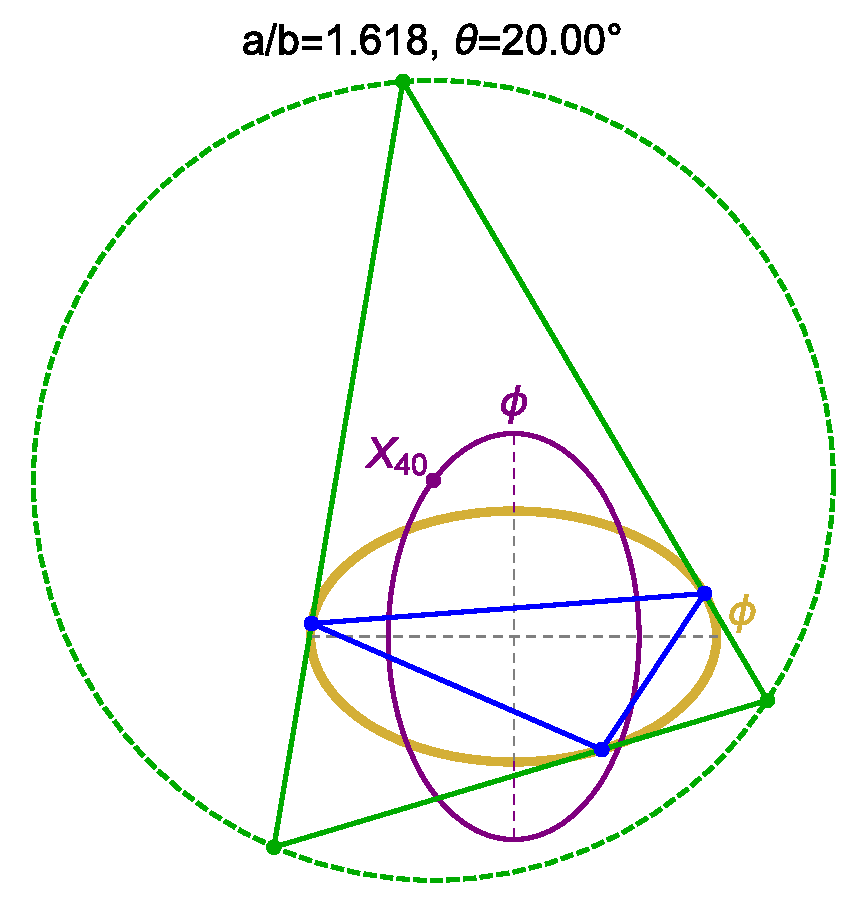
\includegraphics[width=.5\textwidth]{pics/1070_x40.eps}
    \caption{An $a/b=\varphi$ EB is shown golden. Also shown is a sample 3-periodic (blue). The Bevan Point $X_{40}$ is the Circumcenter of the Excentral Triangle (solid green). At this EB aspect ratio, the locus of $X_{40}$ (purple) is a $90^\circ$-rotated copy of the EB. The region common to both ellipses is ${\simeq}70.48\%$ the area of either ellipse. \textbf{Video}: \cite[PL\#13]{reznik2020-playlist-intriguing}.}
    \label{fig:x40-golden}
\end{figure}

\subsection{A Derived Triangle railed onto the EB}

Consider a 3-periodic's Anticomplementary Triangle (ACT) \cite{mw} and its Intouchpoints $i_1^\prime,i_2^\prime,i_3^\prime$, Figure~\ref{fig:act_intouch}. Remarkably:

\begin{theorem}
The locus of the Anticomplementary Triangle's Intouchpoints is the EB.
\end{theorem}

\begin{proof}
Consider an elementary triangle with vertices $Q_1=(0,0)$, $Q_2=(1,0)$  and $Q_3=(u,v)$. Its sides are $s_1=|Q_3-Q_2|$, $s_2=|Q_3-Q_1|$, and $s_3=1$.

Let $E$ be its {\em Circumbilliard}, i.e., the Circumellipse for which ${Q_1}{Q_2}{Q_3}$ is a 3-periodic EB trajectory. The following implicit equation for $E$ was derived \cite{garcia2019-incenter}:

\begin{align*}
 E(x,y)=& v^2 x^2+(u^2+(s_1+s_2-1)u-s_2 )y^2+\\
 &v( 1-s_1-s_2-2u )x y+v(s_2+u)y-v^2x =0
\end{align*}

The vertices of the ACT are given by
 $Q_1^\prime=(u-1,v),\,Q_2^\prime=(u+1,v),\,Q_3^\prime=(1-u,-v)$, and its Incenter\footnote{This is the Nagel Point $X_8$ of the original triangle.} is:
 %
 \begin{equation*}
 X_1^\prime=\left[s_1-s_2+u, \frac{s_2(s_1-1)+(1-s_1+s_2)u  -u^2}{v}
 \right].
 \end{equation*}
 %
 The ACT Intouchpoints are the feet of perpendiculars dropped from $X_1'$ onto each side of the ACT, and can be derived as:
 %
 \begin{align*}
 i_1^\prime=& \left[ \frac{s_1(u-1)u+s_2}{s_2},\frac{ v (s_1-1)}{s_2} \right]\\
  i_2^\prime=& \left[  \frac{ (u-1)(s_2-1)}{s_2}, \frac{(s_2-1)v}{s_2}   \right]\\
   i_3^\prime=& \left[   s_1-s_2+u,v \right].
\end{align*}
 %
Direct calculations shows that
$E(i_1^\prime)=E(i_2^\prime)=E(i_3^\prime)=0.$. Besides always being on the EB, the locus of the Intouchpoints cover it. Let $P_1(t)P_2(t)P_3(t)$ be a 3-periodic and $P_1^{\prime} (t)P_2^{\prime}(t)P_3^{\prime}(t)$ its ACT.
 For all $t$ the Intouchpoint $i_1^{\prime}(t)$ is located on the side $P_2^{\prime}(t) P_3^{\prime}(t)$ of the ACT and on the elliptic arc     $\textrm{arc}(P_1(t)P_3(t))$, Figure \ref{fig:act_intouch}. Therefore, when $P_1(t)$ completes a circuit on the EB, $i_1^{\prime}(t)$ will have to complete a similar tour. 
Analogously for  $i_2^{\prime}(t)$ and  $i_3^{\prime}(t)$.
\end{proof}

\begin{figure}
    \centering
    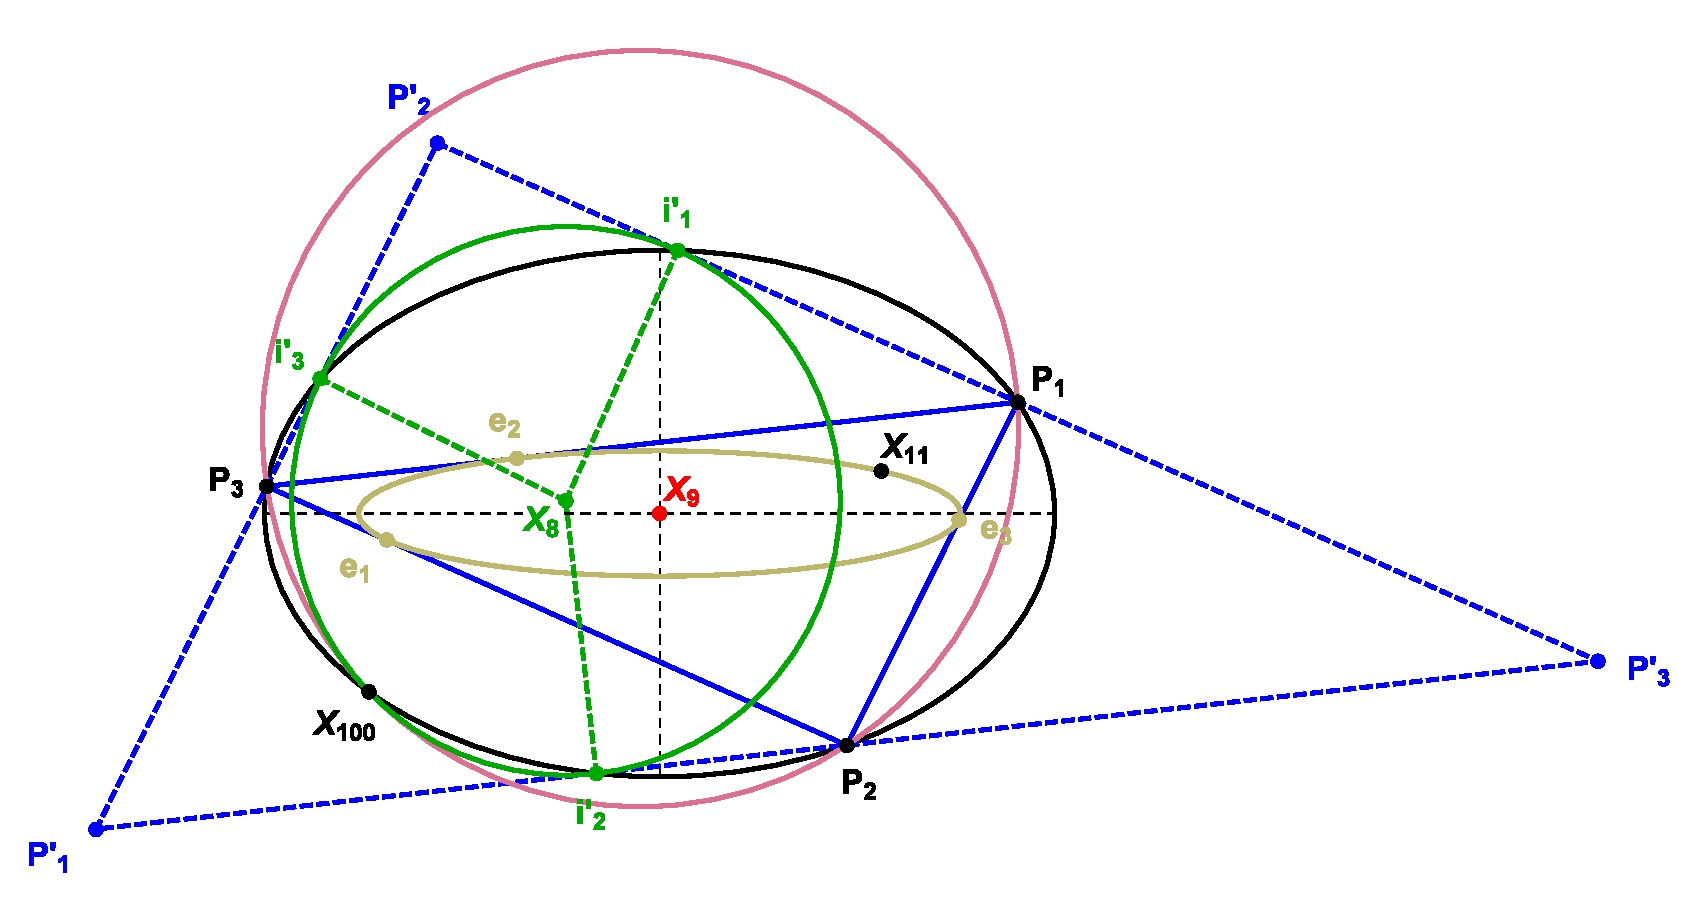
\includegraphics[width=.75\textwidth]{pics/1080_act_intouch.eps}
    \caption{A 3-periodic $P_1P_2P_3$ is shown (blue). Shown also is the Mittenpunkt $X_9$, at the EB center. The 3-periodic's Anticomplementary Triangle (ACT) $P_1'P_2'P_3'$ (dashed blue) has sides parallel to the 3-periodic. The latter's Intouchpoints $i_1'$, $i_2'$, and $i_3'$ are the feet of perpendiculars dropped from the ACT's Incenter ($X_8$) to each side (dashed green). The ACT's Incircle (green) and 9-point circle (the 3-periodic's Circumcircle, pink) meet at $X_{100}$, the ACT's Feuerbach Point. Its locus is also the EB. The Caustic is shown brown. On it there lie $X_{11}$ and the three Extouchpoints $e_1$, $e_2$, $e_3$. \textbf{Video:} \cite[PL\#09]{reznik2020-playlist-intriguing}}
    \label{fig:act_intouch}
\end{figure}
